\documentclass[11pt]{article}
\usepackage{fullpage}
\usepackage{graphicx}
\usepackage{enumitem}
\usepackage{color,soul}
\usepackage{amsmath}
\usepackage[mathletters]{ucs}
\usepackage[utf8x]{inputenc}

\usepackage{tikz}
\usepackage{pgfplots}
\pgfplotsset{compat=1.16}

\usepackage{graphicx}
\graphicspath{{images/}}

\begin{document}
%\newcommand{\answer}[1]{{\bf (Answer: #1)}}
\newcommand{\answer}[1]{\mbox{~}}

{\large  CSCE 464 Wireless and Mobile Systems  \hfill Fall 2019\\
 \begin{center}
   Homework 3 \\
   ({Murtaza Hakimi : 325003943}) \\
    \end{center}
}

Remove all highlights before typing your answer.

\section{802.11}
\begin{enumerate}[label=(\alph*)]
\item {
	802.11 doesn't solve the hidden terminal problem completely but does mitigate it through 
	its request to send (RTS) and clear to send (CTS) mechanisms. It also recommends a higher
	carrier sensing zone which helps.
}
\item {
	The fairness problem is solved by 802.11's back-off mechanism. The mechanism gives a 
	fair share of the overall bandwidth to all stations. 
}
\item {
	Collisions occur in the hidden terminal situation, for example, transmitter 2 can't see a
	transmission from transmitter 1 to router 1 so it will send a packet to router 2 but this would
	collide with transmitter 1's transmission. 
}
\item {
	Roaming happens in layer 2 when a user moves to another access point but stays on the same
	VLAN and the same IP subnet. 
}
\item {
	It varies. A distribution system can be one of three things, a wired network, a switch or a 
	wireless network. A wireless distribution system exists when it is interconnecting access
	points in a WLAN.
}
\item {
	The wi-fi direct technology can be useful for quick and easy connections between devices 
	that are already certified. This "pre-certification" process would also minimize malicious or
	unwanted connections. The features added to 802.11 include avoiding connection to a router
	or access point to connect to another device. 
}
\item {
	Transmission for successful carrier sensing is $2x10^-9 mW$
	
	Physical CS:
	
	Node C:
	$Pt_{AC} = 10^{-11}mW <$ threshold
	$Pt_{BC} = 10^{-9}mW <$ threshold
	
	Node D:
	$Pt_{AD} = 10^{-6}mW >$ threshold
	$Pt_{BD} = 10^{-6}mW >$ threshold
	
	Node E:
	$Pt_{AE} = 10^{-10}mW <$ threshold
	$Pt_{BE} = 10^{-7}mW >$ threshold \\
	
	Virtual CS: (SINR needs to be greater than $25 dBm = 3 x 10^2mW$) 
	
	Node C:
	$Pt_{AC} = 10^{-11}/10^{-10} = 0.1mW < 3 x 10^2mW$
	$Pt_{BC} = 10^{-9}/10^{-10} = 10mW < 3 x 10^2mW$
	
	Node D:
	$Pt_{AD} = 10^{-6}/10^{-10} = 10^{4}mW > 3 x 10^2mW$
	$Pt_{BD} = 10^{-6}/10^{-10} = 10^{4}mW > 3 x 10^2mW$
	
	Node E:
	$Pt_{AE} = 10^{-10}/10^{-10} = 10^{0}mW < 3 x 10^2mW$
	$Pt_{BE} = 10^{-7}/10^{-10} = 10^{3}mW > 3 x 10^2mW$
} 
\end{enumerate}
 


\section{802.11 DCF}
\begin{enumerate}[label=(\alph*)]
\item {
}
\begin{figure}[h] %[h] means "here" You can put [t] for "top"
\centering
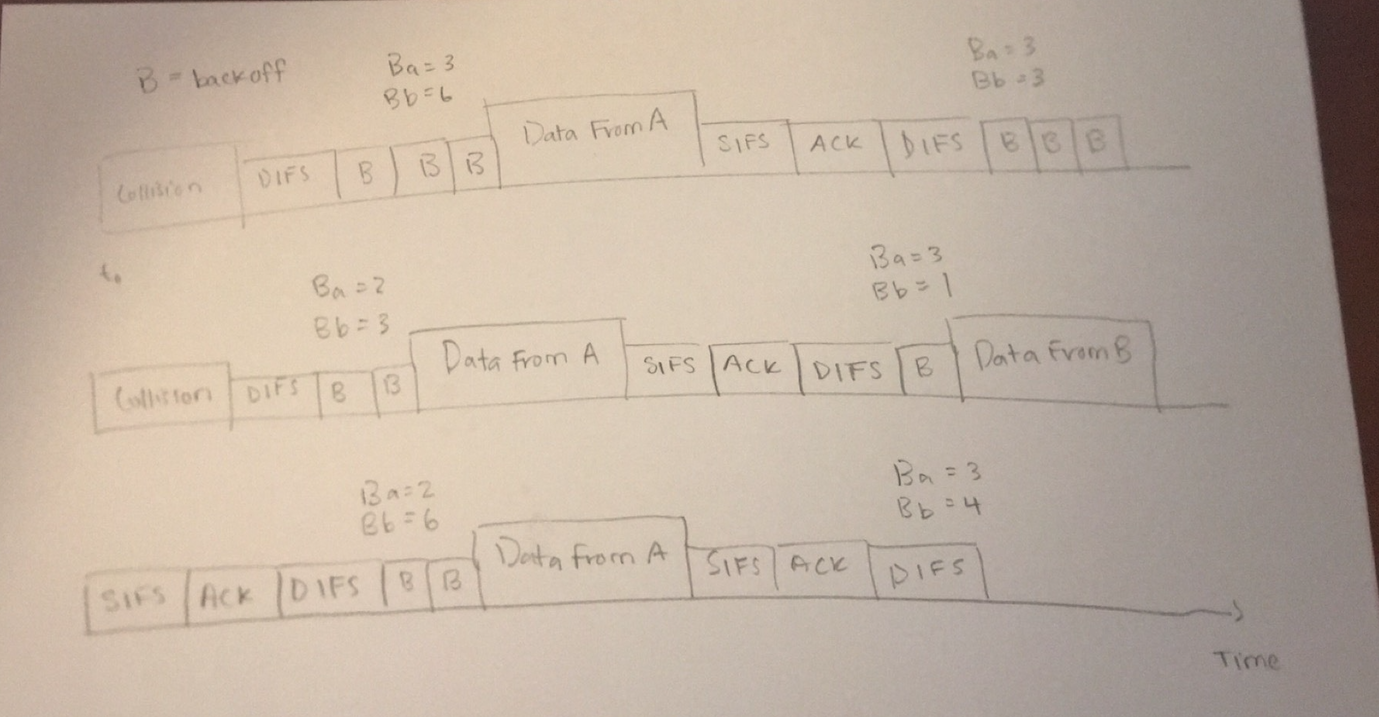
\includegraphics[width=0.5\textwidth]{timeline}
\caption{Timeline}
\end{figure}

\end{enumerate}


\section{Routing}
\begin{enumerate}[label=(\alph*)]
\item {
	One can modify DSR to transmit multiple routes. Unmodified DSR will return the shortest RREQ at the destination when there are multiple broadcasts. The 
	modification though, at destination can send back all other routes to adjust for the misbehaving node. If one of the nodes drops a signal there are other routes 
	that still connect the sender and receiver. 
}
\item {
	No. The approach does not ensure that the source node will discover the shortest route. Suppose there is a network of nodes where A <-> C, A <-> S, A <-> B, 
	S <-> B, B <-> D, D <-> C. If S wants to send a packet to D. S broadcasts a RREQ by appending its address to A and B. If there is high traffic on the path 
	between S and B and the RREQ reaches A first, A will append its address to RREQ and broadcast it to B and C. B hasn't received the RREQ from S so it will
	accept the RREQ from A and when it does eventually receive the RREQ from S it will drop it.
	
	The shortest route would've been SBD but it ended up taking SABD.
}
\item {
	N/A
}
\end{enumerate}

\section{Wireshark}
\begin{enumerate}[label=(\alph*)]
\item {
	In the network, there are two different access points with the \textsc{Bill Clinternet} SSID: \texttt{fc:ec:da:3f:b6:43} and \texttt{80:2a:a8:42:fd:90}.
	
%	\begin{figure}[h]
%		\begin{center}
%			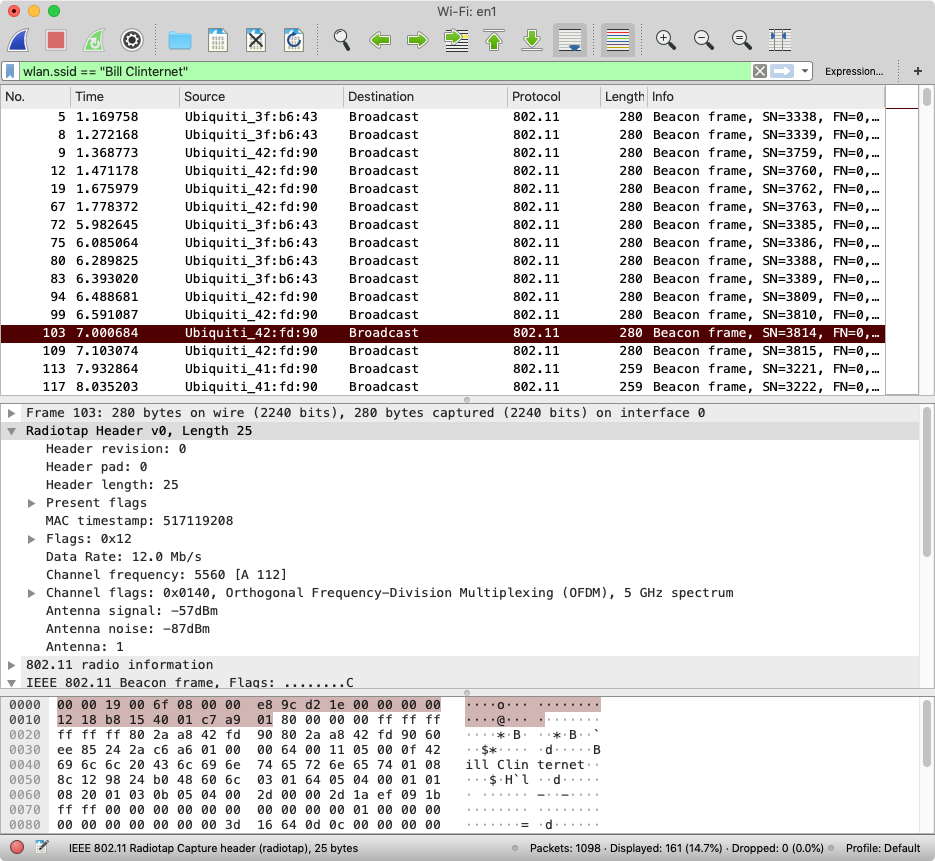
\includegraphics[keepaspectratio,height=6.5cm]{wireshark_4_a.png}
%			\caption{Wireshark screenshot for beacon frames with the \textsc{Bill Clinternet} SSID}
%		\end{center}
%	\end{figure}
	
}
\item {
	The signal strength to the closest access point \texttt{80:2a:a8:42:fd:90} is $-57 \text{dBm}$.
	
%	\begin{figure}[h]
%		\begin{center}
%			\includegraphics[keepaspectratio,height=6.5cm]{wireshark_4_2.png}
%			\caption{Signal strength of a beacon frame received from the access point}
%		\end{center}
%	\end{figure}
}
\item {
	Using the display filter \texttt{wlan.fc.type\_subtype == 0x08} we can show only beacon frames for any nearby access points. This shows the SSIDs \textsc{Bill Clinternet, Hullabaloo Connect Connect, VladimirComputin}. There probably are more access points out there, but they aren't visible because Wireshark does not scan all channels simultaneously.
	
	
	
%	\begin{figure}[h]
%		\begin{center}
%			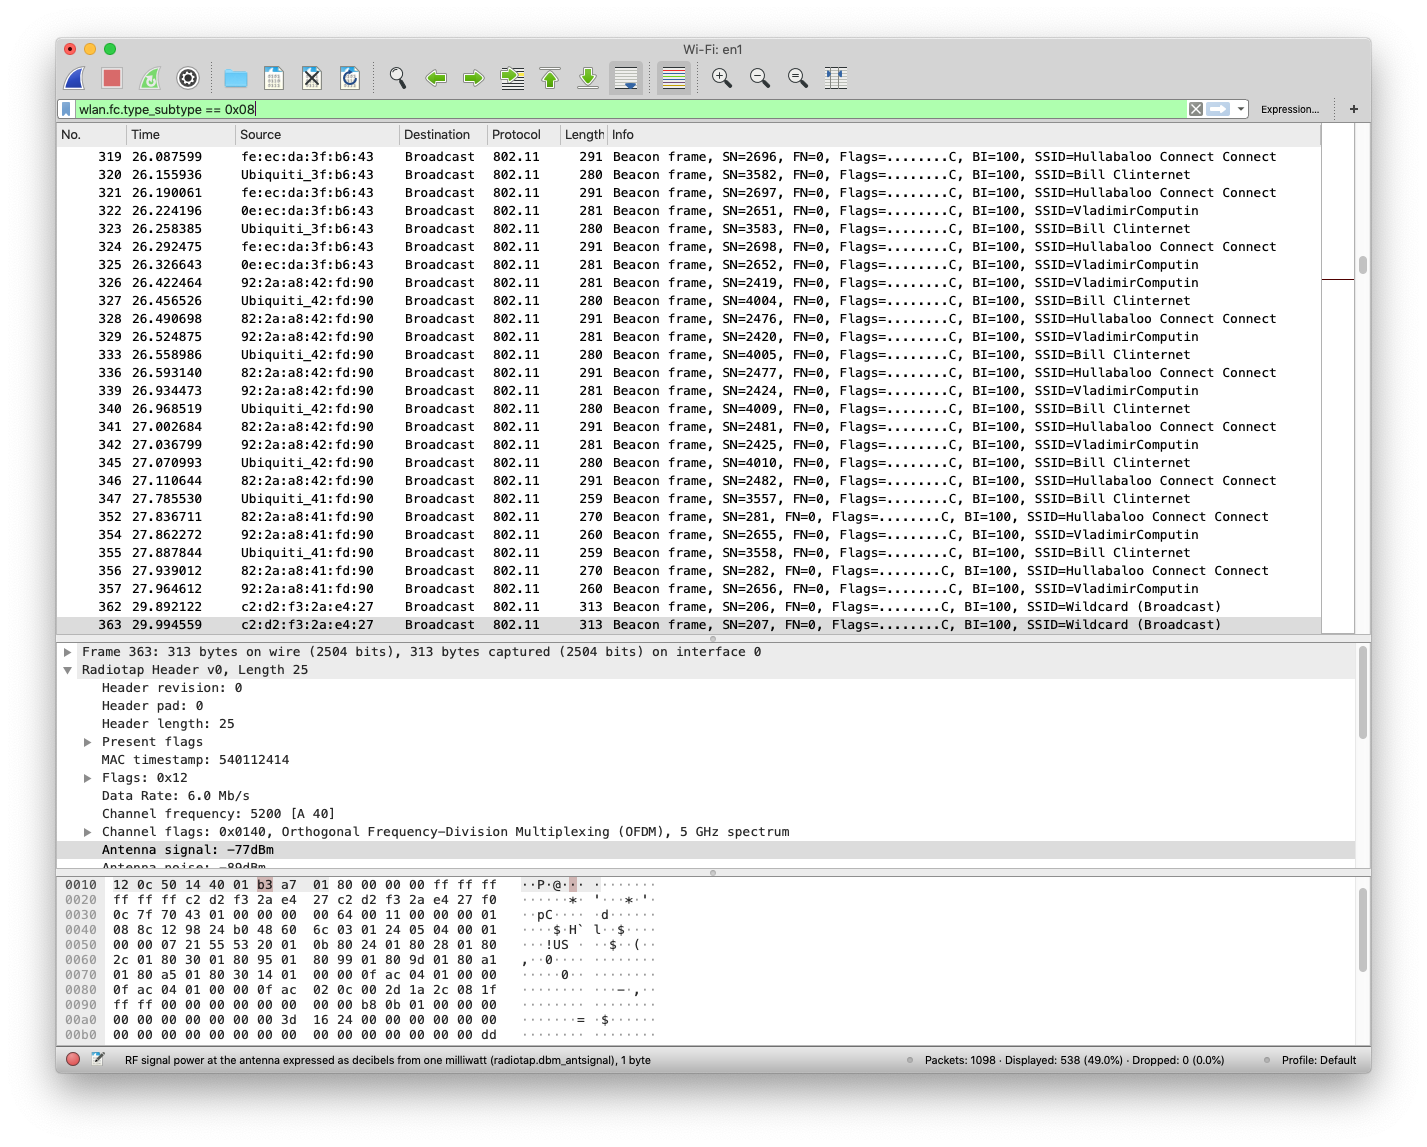
\includegraphics[keepaspectratio,height=6.5cm]{wireshark_4_c.png}
%			\caption{Other access points' beacon frames}
%		\end{center}
%	\end{figure}
}
\end{enumerate}	

\section{Wireshark: RTS/CTS Threshold and Fragmentation Length}
\begin{enumerate}[label=(\alph*)]
\item {
	\textbf{Pre-Experiment Questions}
	\begin{enumerate}
		\item {Advantages of fragmentation include better immunity to noise (since you will resend only a small part of the total payload if noise corrupts it) as well as better, fairer use of air time.}
		\item {For the WNDR3400v2 router, the range of allowable fragmentation lengths is $[256, 2346]$.}
		\item {The smaller the fragmentation length, the higher the protocol overhead (e.g. the ratio of the 802.11 header to the useful payload) will be. If we fragment a packet every 20 bytes, the 802.11 header will take up almost as much time to transmit, making this a very inefficient use of air time.}
	\end{enumerate}
	
	\textbf{Experiment 1}
	\begin{enumerate}
		\item {\textbf{50 byte ICMP packet size}: RTS/CTS frames are sent, the RTS frame is 16 bytes in length and the CTS frame is 10. No fragmentation is used.
			\begin{figure}[h]
				\begin{center}
					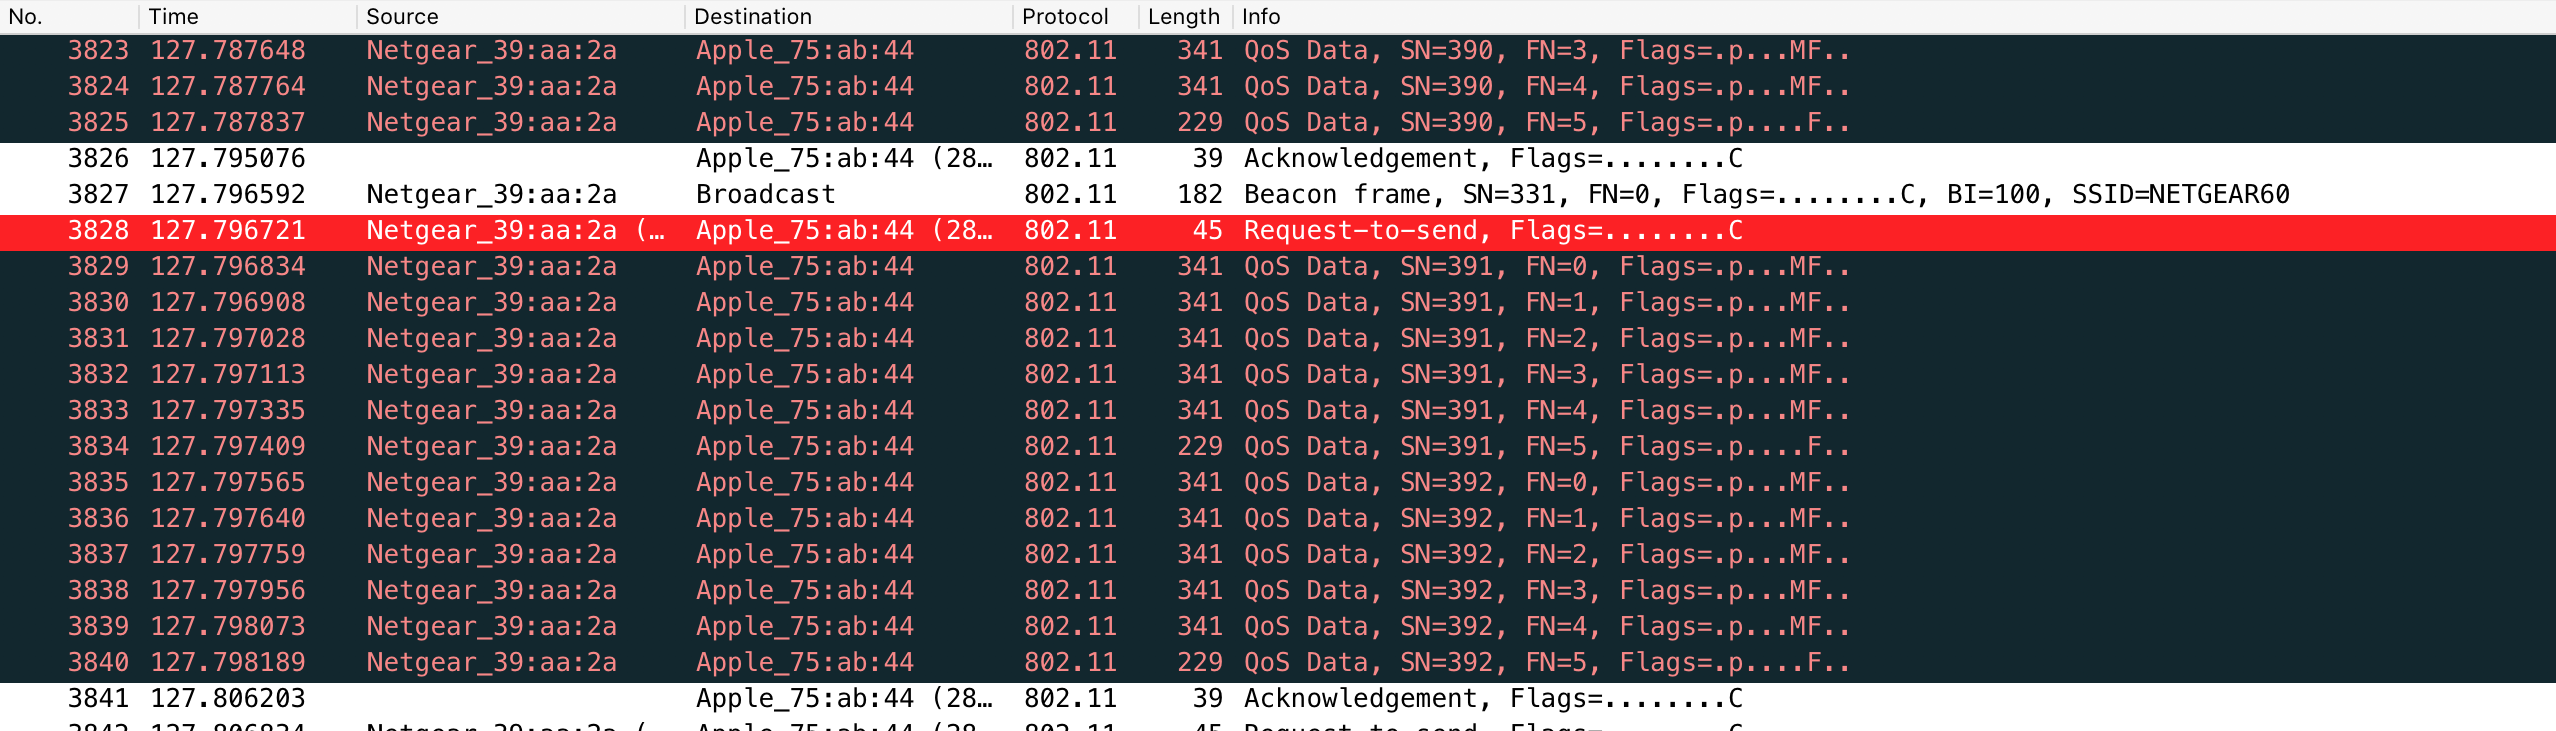
\includegraphics[keepaspectratio,height=4.5cm]{wireshark_5_1_1.png}
				\end{center}
			\end{figure}
		}
		\item {\textbf{300 byte ICMP packet size}: RTS/CTS frames are sent, the RTS frame is 16 bytes in length and the CTS frame is 10. No fragmentation is used.
			\begin{figure}[h]
				\begin{center}
					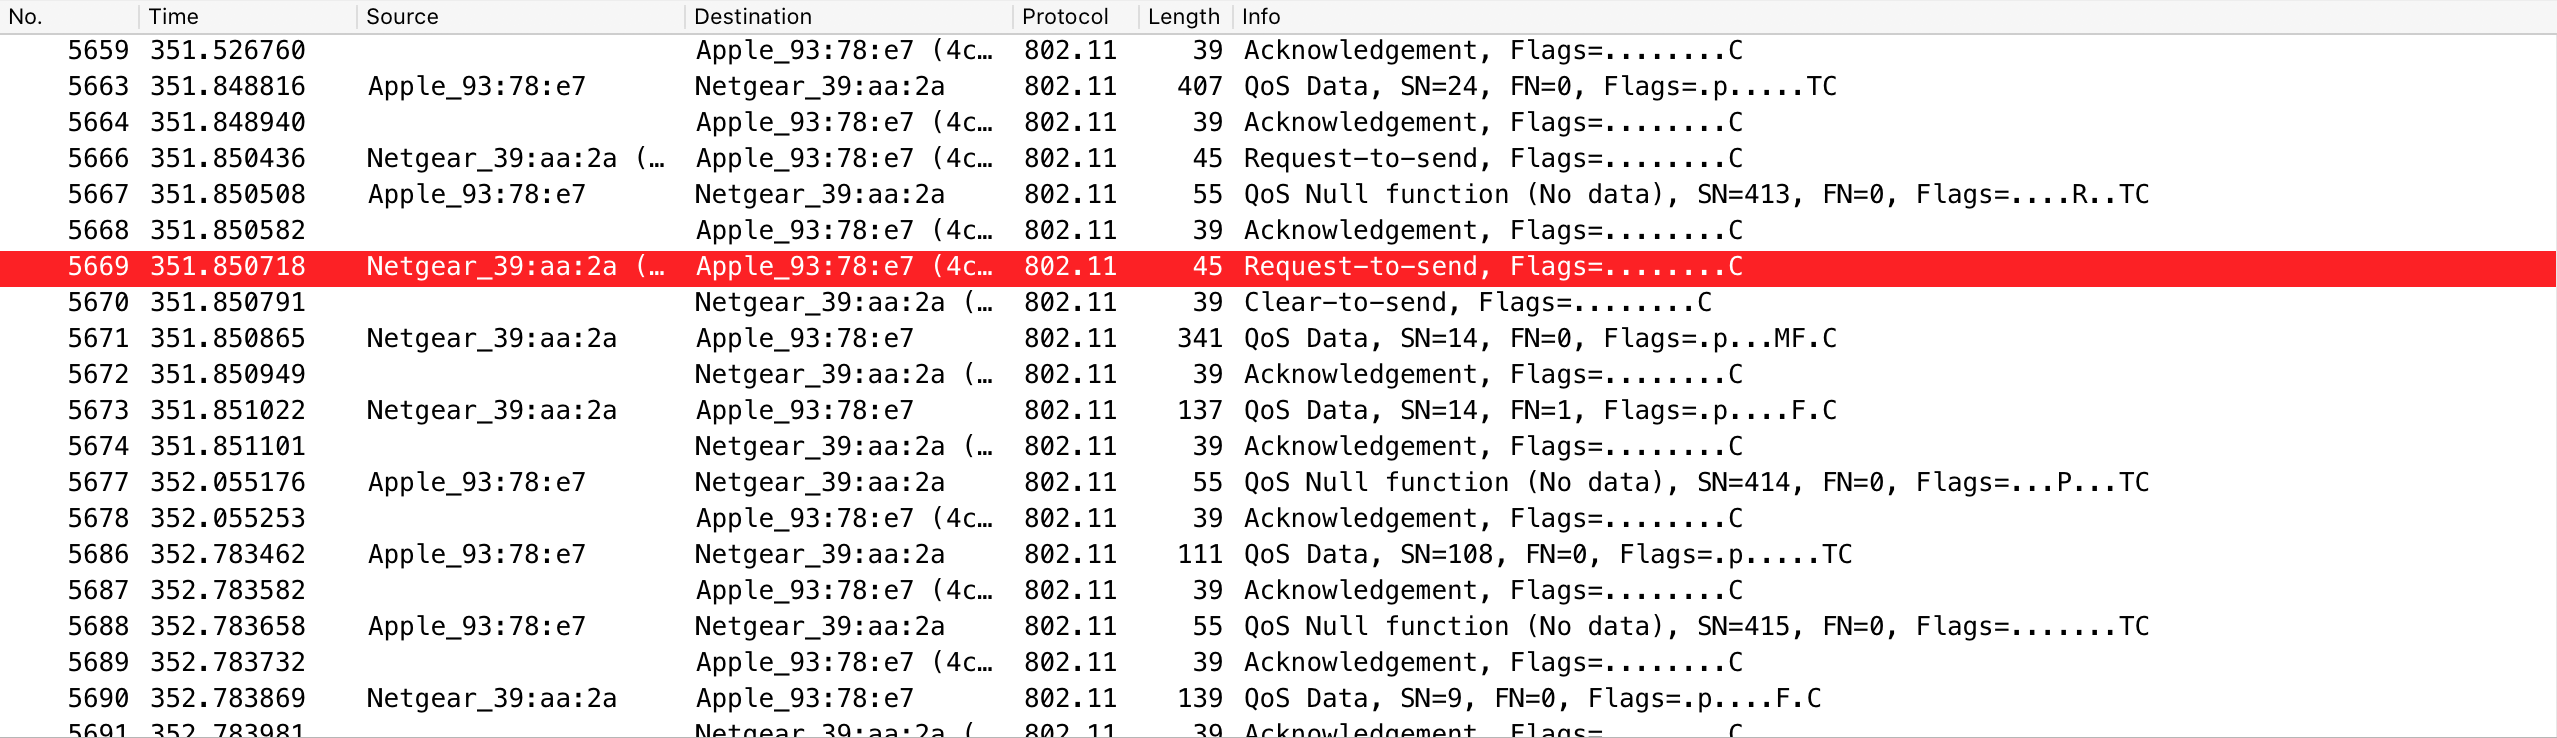
\includegraphics[keepaspectratio,height=4.5cm]{wireshark_5_1_2.png}
				\end{center}
			\end{figure}
		}
		\item {\textbf{600 byte ICMP packet size}: RTS/CTS frames are sent, the RTS frame is 16 bytes in length and the CTS frame is 10. Fragmentation is used as two 300 byte packets typically.
			\begin{figure}[h]
				\begin{center}
					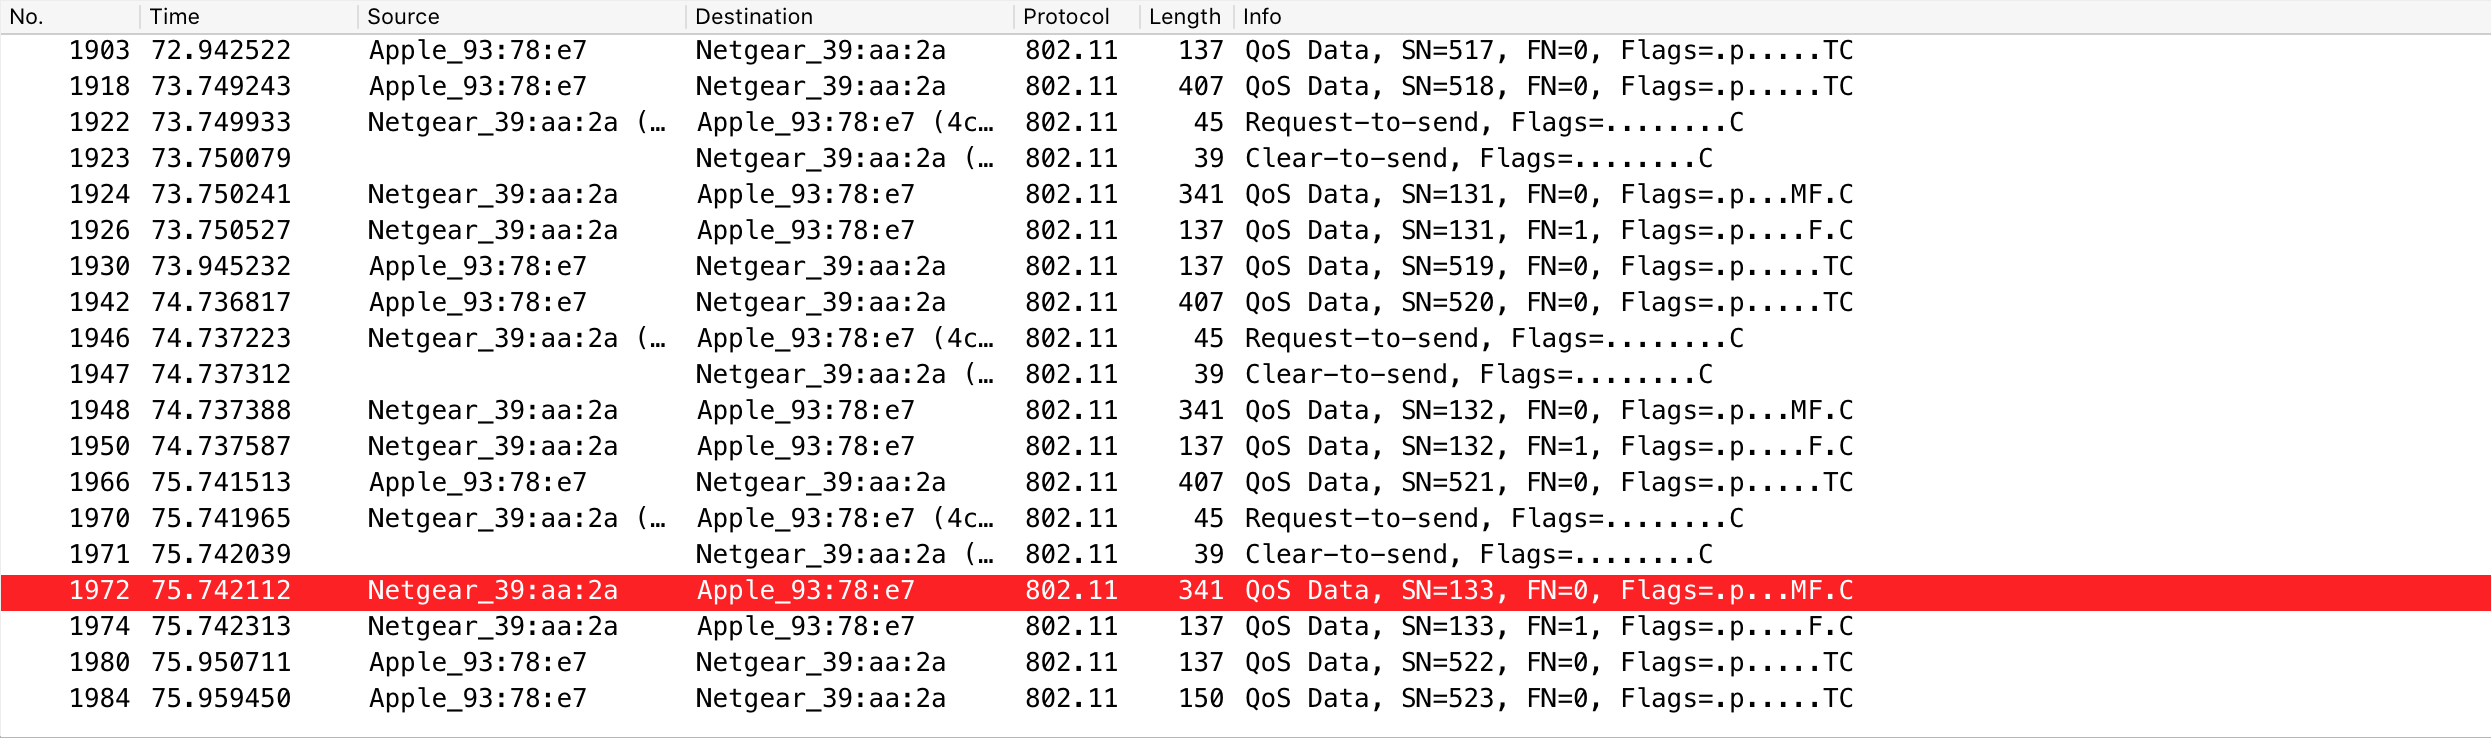
\includegraphics[keepaspectratio,height=4.5cm]{wireshark_5_1_3.png}
				\end{center}
			\end{figure}
		}
		
		\item {\textbf{1200 byte ICMP packet size}: RTS/CTS frames are sent, the RTS frame is 16 bytes in length and the CTS frame is 10. There are 6 fragments, the first 5 of which carry 278 bytes of payload, the last 94 bytes.
			\begin{figure}[h]
				\begin{center}
					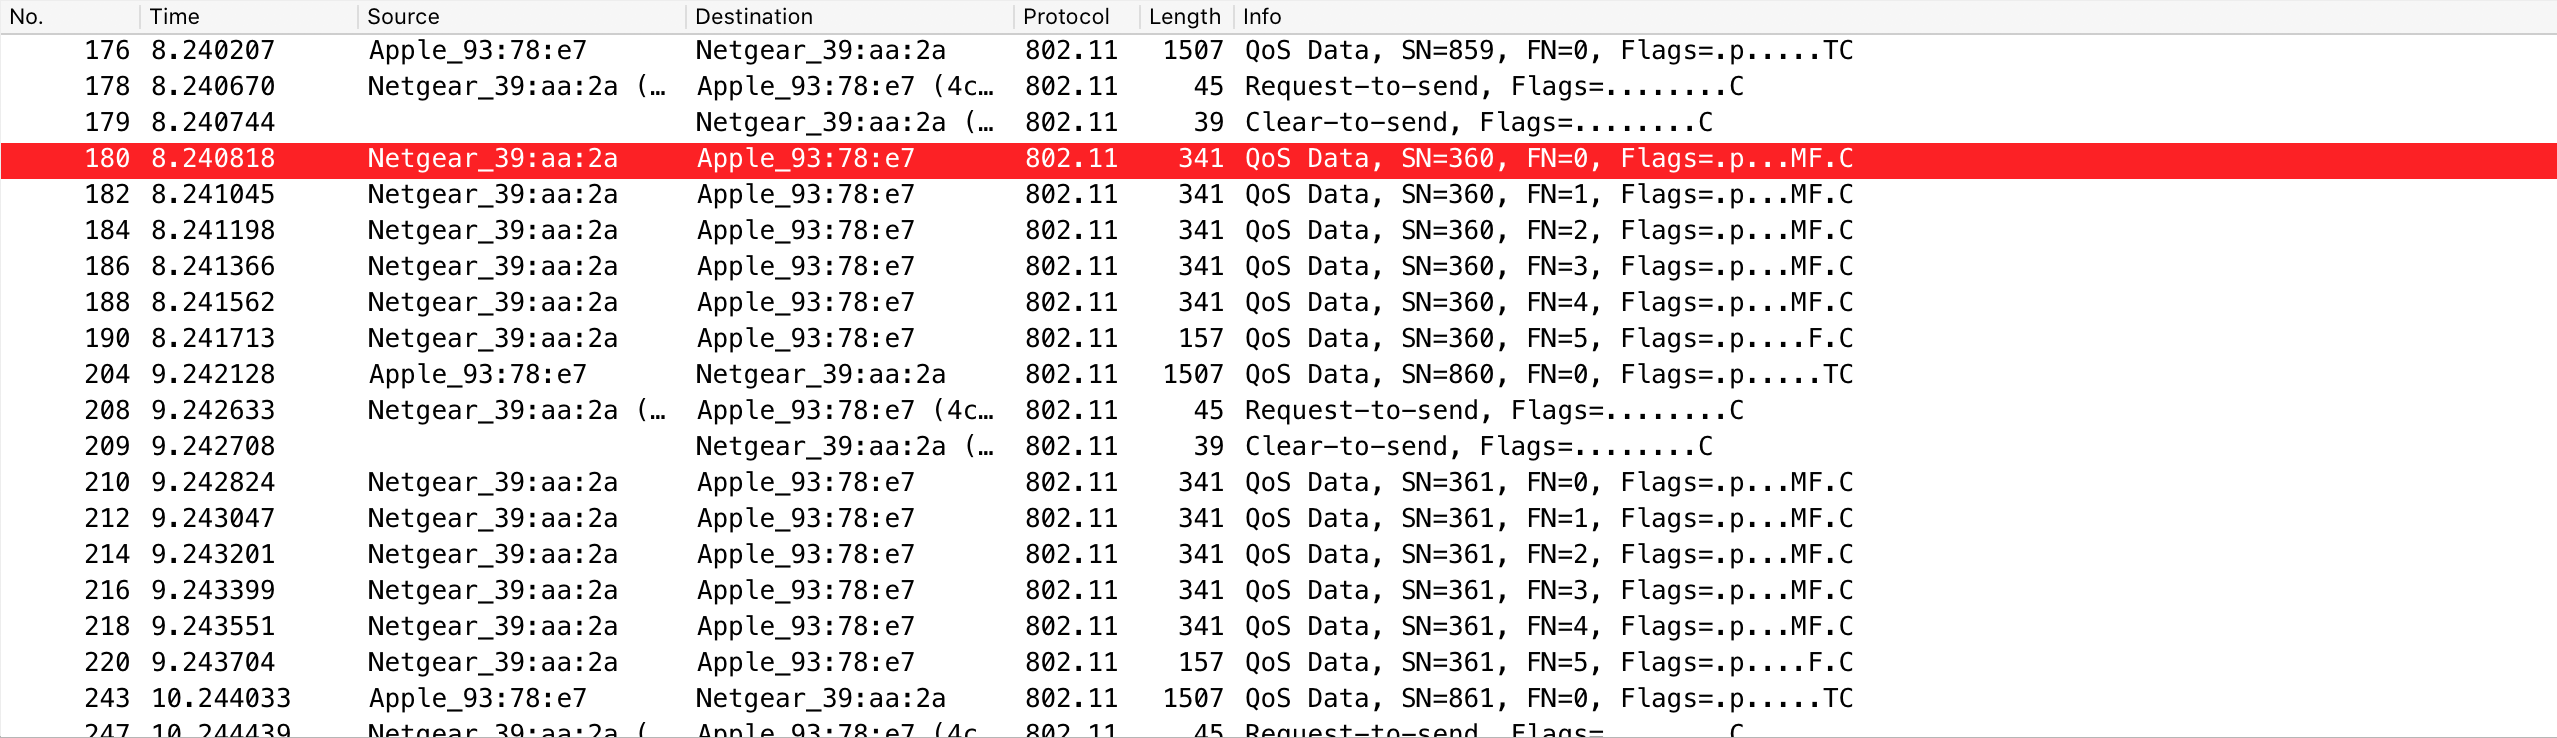
\includegraphics[keepaspectratio,height=4.5cm]{wireshark_5_1_4.png}
				\end{center}
			\end{figure}
		}
	\end{enumerate}
}
\item {
	\textbf{Experiment 2} \\
	
\begin{tabular}{|l|l|}
\multicolumn{2}{c}{100 bytes, 200µS} \\
\hline
\textbf{Packet loss} & \textbf{RTT (mS)} \\ \hline
98\% & 40 \\
98\% & 50.8 \\
97\% & 63.1 \\
98\% & 56.8 \\
99\% & 59.9 \\
\hline
98.0\% & 54.12 \\ 
\hline
\end{tabular}
\begin{tabular}{|l|l|}
\multicolumn{2}{c}{100 bytes, 500µS} \\
\hline
\textbf{Packet loss} & \textbf{RTT (mS)} \\ \hline
95\% & 126.3 \\
96\% & 121.2 \\
95\% & 152.3 \\
96\% & 143.1 \\
96\% & 133.8 \\
\hline
95.6\% & 135.34 \\
\hline
\end{tabular}
\begin{tabular}{|l|l|}
\multicolumn{2}{c}{100 bytes, 1000µS} \\
\hline
\textbf{Packet loss} & \textbf{RTT (mS)} \\ \hline
86\% & 243.5 \\
83\% & 234.8 \\
85\% & 239.3 \\
86\% & 240.3 \\
83\% & 243.3 \\
\hline
85\% & 240.24 \\
\hline
\end{tabular}


	
\begin{tabular}{|l|l|}
\multicolumn{2}{c}{1000 bytes, 200µS} \\
\hline
\textbf{Packet loss} & \textbf{RTT (mS)} \\ \hline
97\% & 42.5 \\
98\% & 60.5 \\
97\% & 49.3 \\
98\% & 50.7 \\
98\% & 57.3 \\
\hline
98\% & 52.06 \\ 
\hline
\end{tabular}
\begin{tabular}{|l|l|}
\multicolumn{2}{c}{1000 bytes, 500µS} \\
\hline
\textbf{Packet loss} & \textbf{RTT (mS)} \\ \hline
94\% & 158.5 \\
95\% & 147.2 \\
94\% & 149.7 \\
96\% & 152.3 \\
94\% & 159.1 \\
\hline
95\% & 153.36 \\
\hline
\end{tabular}
\begin{tabular}{|l|l|}
\multicolumn{2}{c}{1000 bytes, 1000µS} \\
\hline
\textbf{Packet loss} & \textbf{RTT (mS)} \\ \hline
84\% & 256.3 \\
90\% & 250.9 \\
88\% & 251.7 \\
87\% & 249.3 \\
90\% & 243.3 \\
\hline
88\% & 250.3 \\
\hline
\end{tabular}
	}
\end{enumerate}



\end{document}

